%\documentclass{beamer}
%\usetheme{Pittsburgh}
\documentclass{scrartcl}

\usepackage[utf8]{inputenc}
\usepackage{default}
\usepackage[procnames]{listings}
\usepackage{graphicx}
%\usepackage[toc,page]{appendix}
\usepackage{caption}
\usepackage{hyperref}
\usepackage{color}
%\usepackage{csvsimple}
\usepackage{float}
\usepackage[T1]{fontenc}



%Bibliogrpahy?
\usepackage{bibentry}
%\nobibliography*
%\bibentry{ }


%Python
\definecolor{keywords}{RGB}{255,0,90}
\definecolor{comments}{RGB}{0,0,113}
\definecolor{red}{RGB}{160,0,0}
\definecolor{green}{RGB}{0,150,0}
\lstset{language=Python,
    basicstyle=\ttfamily\scriptsize,
    keywordstyle=\color{keywords},
    commentstyle=\color{comments},
    stringstyle=\color{red},
    identifierstyle=\color{green},
    breaklines = true,
    columns=fullflexible,
    %Numbering and tabs
    %numbers=left,
    %numberstyle=\tiny\color{gray},
    %stepnumber=2,
    %numbersep=1em,
    tabsize=4,
    showspaces=false,
    showstringspaces=false}

\begin{document}

\title{Scientific Experimentation and Evaluation
}
\subtitle{
Assignment: 3.1}
\author{
  Matin, Maryam \\
  Quignon, Christophe
  %Familyname, Name
}
\date{\today}


\maketitle


\section{Description of the calibration process}

\subsection{Overall process}
\paragraph{Description}

In this assignment we executed the camera calibration script which we had previously implemented using python-OpenCV library. We used a set of camera captured images from our own printed pattern which is an 8x8 square checkerboard (the length of each square is 2 cm).\\

We fixed and sticked the pattern to a clip pad to ensure the pattern was completely flat. We pointed the camera downwards and placed it at a fixed position. The resolution of the camera was also set to Full HD (1920 x 1080 pixels). We then tried to capture images by moving the pattern in front of the camera. We placed the pattern at different poses in such a way that it covers different  possible orientations and distances in camera's field of view. As discussed before we start with an orthogonal view and then two rotations with roughly 30 $^\circ $ on every axis of the frame.\\

The Python-OpenCV implementation of camera calibration doesn't provide us with error estimates and only gives information about the initial and new calibrated camera matrices, rotation and translation matrices, distortion coefficients and region of interest and also a return value which says whether the checkerboard was found or not. However these information were still enough to have an estimation of the accuracy of the calibration process.\\


The intrinsic parameters of the camera which are unique to each camera and hence can be used in the future include information about focal length and the principal (optical) point (usually at the center of the image). The first two elements of the old and new camera matrices in the first and second columns represent the focal length and the values on the third column represent the principal point of the camera. \\

As discussed in the class, before starting the experiments we turned on the camera and let it warm up for an hour and then turned it off to cool it down. We started taking our images after turning it on again and when it got back to the steady state. Luckily we didn't face any auto-focusing issues. We did the calibration process 2 times and for 2 different image sets and recorded our findings. At each turn we captured almost 20 different images.\\



\section{First Experiment}

\subsection{Output}

In our first experiment the brightness of the images were high and the following results were achieved (See run1.txt) :\\


\lstinputlisting{run1.txt} 



\subsection{Analysis}

As it can be seen here the pattern corners were detected for 15 images. In this experiment we observed more differences between the values of the fx and fy in the calibrated camera matrix in comparision to the initial camera matrix. We also expected the RoI to be almost the size of the original image but the numbers were far different than the original frame size.\\



\paragraph{Problem}
\begin{itemize}
\item The problem here was that since the images were too bright, at some points the brightness makes the grid appear such that the corners are not touching each other so the detection becomes imprecise. Fig. 1 illustrates this finding.\\
\end{itemize}



\begin{figure}[H]
\centering
\begin{minipage}{.5\textwidth}
  \centering
  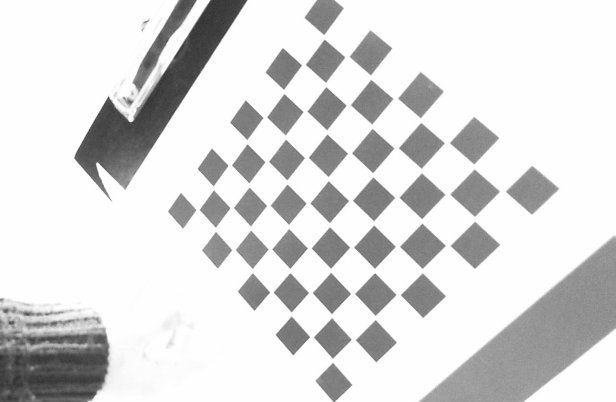
\includegraphics[width=.8\linewidth]{img/brightness.jpg}
  %\caption{}
  %\label{fig:}
\end{minipage}%
\begin{minipage}{.5\textwidth}
  \centering
  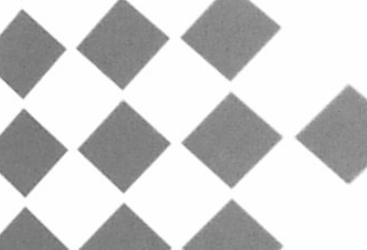
\includegraphics[width=.8\linewidth]{img/bright_detail.jpg}
  %\caption{}
  %\label{fig:} 
\end{minipage}
\caption{Sample of highly brightened images (left) and its detailed view (right)}
\label{fig:brightness}
\end{figure}



\section{Second Experiment}

\subsection{Output}

In the second run, we reduced the brightness of the images and repeated image capturing. We captured 22 images out of which in 18 cases the corners were detected. Fig. 2 represents the images captured and the detected corners for these images. The outputs of the calibration are represented below: (See also test.txt)\\
 
\lstinputlisting{test.txt} 



\subsection{Analysis}

In this experiment the results of the focal lengths obtained for the new camera matrix are  closer to each other than the original camera matrix so it is more centered. We can also see that the RoI is closer to the original image size and hence we have had less distortions to be cut off.\\

%images

\begin{figure}[H]
\centering
\begin{minipage}{.5\textwidth}
  \centering
  \includegraphics[width=1.0\linewidth]{img/1.jpeg}
  %\caption{}
  %\label{fig:}
\end{minipage}
\begin{minipage}{.5\textwidth}
  \centering
  \includegraphics[width=1.0\linewidth]{img/2.jpeg}
  %\caption{}
  %\label{fig:}
\end{minipage}
\begin{minipage}{.5\textwidth}
  \centering
  \includegraphics[width=1.0\linewidth]{img/3.jpeg}
  %\caption{}
  %\label{fig:}
\end{minipage}
\begin{minipage}{.5\textwidth}
  \centering
  \includegraphics[width=1.0\linewidth]{img/4.jpeg}
  %\caption{}
  %\label{fig:}
\end{minipage}
\begin{minipage}{.5\textwidth}
  \centering
  \includegraphics[width=1.0\linewidth]{img/5.jpeg}
  %\caption{}
  %\label{fig:}
\end{minipage}
\begin{minipage}{.5\textwidth}
  \centering
  \includegraphics[width=1.0\linewidth]{img/6.jpeg}
  %\caption{}
  %\label{fig:}
\end{minipage}
\begin{minipage}{.5\textwidth}
  \centering
  \includegraphics[width=1.0\linewidth]{img/8.jpeg}
  %\caption{}
  %\label{fig:}
\end{minipage}
\begin{minipage}{.5\textwidth}
  \centering
  \includegraphics[width=1.0\linewidth]{img/9.jpeg}
  %\caption{}
  %\label{fig:}
\end{minipage}
\begin{minipage}{.5\textwidth}
  \centering
  \includegraphics[width=1.0\linewidth]{img/10.jpeg}
  %\caption{}
  %\label{fig:}
\end{minipage}

%\caption{Histograms of the angles and distances of the right run.}
\end{figure}



\begin{figure}[H]
\centering
\begin{minipage}{.5\textwidth}
  \centering
  \includegraphics[width=1.0\linewidth]{img/11.jpeg}
  %\caption{}
  %\label{fig:}
\end{minipage}
\begin{minipage}{.5\textwidth}
  \centering
  \includegraphics[width=1.0\linewidth]{img/12.jpeg}
  %\caption{}
  %\label{fig:}
\end{minipage}
\begin{minipage}{.5\textwidth}
  \centering
  \includegraphics[width=1.0\linewidth]{img/13.jpeg}
  %\caption{}
  %\label{fig:}
\end{minipage}
\begin{minipage}{.5\textwidth}
  \centering
  \includegraphics[width=1.0\linewidth]{img/14.jpeg}
  %\caption{}
  %\label{fig:}
\end{minipage}
\begin{minipage}{.5\textwidth}
  \centering
  \includegraphics[width=1.0\linewidth]{img/16.jpeg}
  %\caption{}
  %\label{fig:}
\end{minipage}
\begin{minipage}{.5\textwidth}
  \centering
  \includegraphics[width=1.0\linewidth]{img/17.jpeg}
  %\caption{}
  %\label{fig:}
\end{minipage}
\begin{minipage}{.5\textwidth}
  \centering
  \includegraphics[width=1.0\linewidth]{img/18.jpeg}
  %\caption{}
  %\label{fig:}
\end{minipage}
\begin{minipage}{.5\textwidth}
  \centering
  \includegraphics[width=1.0\linewidth]{img/19.jpeg}
  %\caption{}
  %\label{fig:}
\end{minipage}
\begin{minipage}{.5\textwidth}
  \centering
  \includegraphics[width=1.0\linewidth]{img/21.jpeg}
  %\caption{}
  %\label{fig:}
\end{minipage}

\caption{Captured images (left) and their detected corners (right)}
\end{figure}


Therefore, in general we can conclude that the second calibrated camera matrix is better to be as our camera model.\\

\section{General possible errors and pitfalls}

\begin{itemize}
\item The camera is very light sensitive. It works best at low light. Lighting conditions can make the pattern indistinguishable
\item The camera frame must not move.
\item The calibration pattern may be scaled or even distorted during the printing procedure.
\item The calibration pattern must be flat and not curved
\item The background must not contain patterns similar to the calibration pattern.
\item It is important to release the camera after taking an image, otherwise it will stay blocked
\item When the captured imaged is stored, compression should not distort the calibration pattern.
\item The lens has to be clean.
\end{itemize}



%\paragraph{Experiment}
%problems while testing including problems with laptop/camera

%The camera connected without any issues

%One has to make sure which index to use, because the index destinguished between the built-in camera of the laptop and the usb camera


\section{Appendix}

\subsection{cam2jpg.py}
\lstinputlisting[language=Python]{cam2jpg.py}


\subsection{calibration.py}
\lstinputlisting[language=Python]{calibration.py}




%BIBLIOGRPAHY!
\bibliographystyle{plain}%amsalpha
\bibliography{bib.bib}
%\bibentry{}


%COPY AND PASTE FROM HERE

%\begin{enumerate}
% \item
%\end{enumerate}

%\href{link}{text}

%\begin[Language=Python]{lstlisting}
%#PYTHON CODE HERE
%\end{lstlisting}

%\lstinputlisting[language=Java]{ }

%\csvautotabular[separator=semicolon]{data.csv}

%\begin{figure}
% \center
% \includegraphics[width= cm]{img/ }
% \caption{}
%\end{figure}



\end{document}
